The \peripheral{TIMERx} peripheral is a 32-bit general purpose timer/counter unit with glitch-free clock source switching. Its main features are listed below:

\begin{itemize}
	\item 32-bit timer values, from 0 to 4,294,967,295
	\item Memory mapped register to read and write current timer value
	\item Three output compare units, two of which can generate pulse width modulation (PWM) waveforms
	\item Two input capture units for precise timing measurements of external signals
	\item Four clock sources: SMCLK, MCLK, LFXT, HFXT
	\item Configurable clock divider (÷1 to ÷32,768)
	\item Glitch-free clock source multiplexer
	\item Six separate interrupts: 2 capture, 3 compare, 1 overflow
	\item Latched register reads for noise immunity
\end{itemize}



\subsection{Timer Pins}

The \peripheral{TIMERx} peripheral has four pins: \pin{TxCMP0}, \pin{TxCMP1}, \pin{TxCAP0}, and \pin{TxCAP1}.

The \pin{TxCMP0} pin outputs the PWM waveform generated by the output compare unit 0. When the corresponding \register{PxSEL[y]} bit is a 1, the \peripheral{TIMERx} peripheral seizes the \texttt{DIR}, \texttt{OUT}, and \texttt{REN} controls of the pin, forcing it to be in output mode. Similarly, \pin{TxCMP1} outputs the PWM waveform of output compare unit 1.

The \pin{TxCAP0} pin is an input that waits for a pin state change and then notifies the input capture unit 0, allowing precise timing of pin changes. The corresponding \register{PxSEL[y]} bit has no effect on this pin, since its secondary/peripheral function only ever acts as an input. Similarly, \pin{TxCAP1} is attached to input capture unit 1.



\subsection{Clock Sources and Divider}

\begin{figure}[htpb]
	\centering
	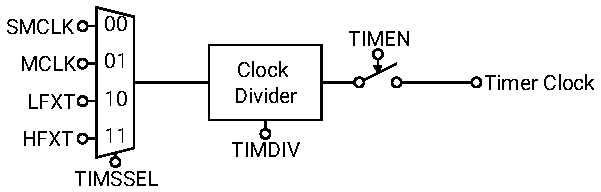
\includegraphics{figures/timer-clock-diagram.pdf}
	\caption{\peripheral{TIMERx} Clock Diagram}
	\label{fig:timer-clock-diagram}
\end{figure}

The clock source for the \peripheral{TIMERx} peripheral can be selected using \bitfield{TSSEL} from four options: SMCLK, MCLK, LFXT (low frequency external clock), and HFXT (high frequency external clock). A glitch-free clock multiplexer built into the clock source selector prevents spurious clock transitions on the timer clock, allowing the user to switch clock sources freely even while the timer is enabled. However, switching clocks will cause the timer clock to be inactive for several clock cycles of the clock that is being switched from or to, whichever has a smaller frequency.

After the clock multiplexer, the timer clock frequency may optionally be reduced with a clock divider controlled by \bitfield{TDIV}. The timer value register \register{TIMxVAL} increments by 1 on every rising edge of the divided timer clock when \peripheral{TIMERx} is enabled with \bitfield{TEN}.

A clock diagram for the \peripheral{TIMERx} peripheral is shown in Figure \ref{fig:timer-clock-diagram}.



\subsection{Starting, Halting, Setting, and Reading the Timer}

To start the timer, set the \bitfield{TEN} bit to 1, whereupon the timer will begin incrementing by 1 with each rising edge of the divided timer clock. To halt the timer at its present value, clear the \bitfield{TEN} bit to 0. The timer will retain its value until it is enabled again, its value is set manually, or the MCU is reset. If the timer is reenabled, it will begin counting from the timer value just before it was reenabled.

The timer value may be manually set at any time by writing the new 32-bit timer value to the \register{TIMxVAL} register. The timer value is updated immediately, regardless of if the timer is enabled or disabled.

The timer value may be read at any time by reading its value from the \register{TIMxVAL} register, regardless of if the timer is enabled or disabled. The \register{TIMxVAL} register is latched on the falling edge of the memory enable signal for stable reads during timer operation.



\subsection{Overflow and Rollover Behavior}

When the timer is enabled and its 32-bit value reaches its maximum of 4,294,967,295, the value will roll over back to zero on the next rising edge of the timer clock and the timer overflow interrupt flag \bitfield{TOVIF} will be set. The timer will then continue incrementing as normal.

Optionally, the user may configure the timer to roll over before the 32-bit limit is reached by setting the new rollover value in the \register{TIMxCMP2} register and setting the \bitfield{TCMP2RST} bit to 1. In this mode, when the timer value becomes equivalent to the value of \register{TIMxCMP2}, the timer value will roll over back to zero on the next rising edge of the timer clock and then continue incrementing as normal, as depicted in Figure \ref{fig:timer-rollover-operation}. This mechanism is used for setting the period of the PWM signals for the output compare units. Note: the timer rolls over back to zero when its value is \textit{equal} to that of \register{TIMxCMP2}, but not if its value is greater than \register{TIMxCMP2}. This becomes important if the user manually sets the timer value above \register{TIMxCMP2}, or if the user sets \register{TIMxCMP2} below the current timer value, whereupon the timer will continue counting all the way to the 32-bit maximum value.

\begin{figure}[htpb]
	%% Creator: Matplotlib, PGF backend
%%
%% To include the figure in your LaTeX document, write
%%   \input{<filename>.pgf}
%%
%% Make sure the required packages are loaded in your preamble
%%   \usepackage{pgf}
%%
%% and, on pdftex
%%   \usepackage[utf8]{inputenc}\DeclareUnicodeCharacter{2212}{-}
%%
%% or, on luatex and xetex
%%   \usepackage{unicode-math}
%%
%% Figures using additional raster images can only be included by \input if
%% they are in the same directory as the main LaTeX file. For loading figures
%% from other directories you can use the `import` package
%%   \usepackage{import}
%%
%% and then include the figures with
%%   \import{<path to file>}{<filename>.pgf}
%%
%% Matplotlib used the following preamble
%%   \usepackage{fontspec}
%%
\begingroup%
\makeatletter%
\begin{pgfpicture}%
\pgfpathrectangle{\pgfpointorigin}{\pgfqpoint{5.000000in}{1.312500in}}%
\pgfusepath{use as bounding box, clip}%
\begin{pgfscope}%
\pgfsetbuttcap%
\pgfsetmiterjoin%
\pgfsetlinewidth{0.000000pt}%
\definecolor{currentstroke}{rgb}{0.000000,0.000000,0.000000}%
\pgfsetstrokecolor{currentstroke}%
\pgfsetstrokeopacity{0.000000}%
\pgfsetdash{}{0pt}%
\pgfpathmoveto{\pgfqpoint{0.000000in}{0.000000in}}%
\pgfpathlineto{\pgfqpoint{5.000000in}{0.000000in}}%
\pgfpathlineto{\pgfqpoint{5.000000in}{1.312500in}}%
\pgfpathlineto{\pgfqpoint{0.000000in}{1.312500in}}%
\pgfpathclose%
\pgfusepath{}%
\end{pgfscope}%
\begin{pgfscope}%
\pgfsetbuttcap%
\pgfsetmiterjoin%
\pgfsetlinewidth{0.000000pt}%
\definecolor{currentstroke}{rgb}{0.000000,0.000000,0.000000}%
\pgfsetstrokecolor{currentstroke}%
\pgfsetstrokeopacity{0.000000}%
\pgfsetdash{}{0pt}%
\pgfpathmoveto{\pgfqpoint{1.000000in}{0.196875in}}%
\pgfpathlineto{\pgfqpoint{4.250000in}{0.196875in}}%
\pgfpathlineto{\pgfqpoint{4.250000in}{1.207500in}}%
\pgfpathlineto{\pgfqpoint{1.000000in}{1.207500in}}%
\pgfpathclose%
\pgfusepath{}%
\end{pgfscope}%
\begin{pgfscope}%
\definecolor{textcolor}{rgb}{0.000000,0.000000,0.000000}%
\pgfsetstrokecolor{textcolor}%
\pgfsetfillcolor{textcolor}%
\pgftext[x=2.625000in,y=0.141319in,,top]{\color{textcolor}\rmfamily\fontsize{8.000000}{9.600000}\selectfont Time}%
\end{pgfscope}%
\begin{pgfscope}%
\pgfsetbuttcap%
\pgfsetroundjoin%
\definecolor{currentfill}{rgb}{0.000000,0.000000,0.000000}%
\pgfsetfillcolor{currentfill}%
\pgfsetlinewidth{0.803000pt}%
\definecolor{currentstroke}{rgb}{0.000000,0.000000,0.000000}%
\pgfsetstrokecolor{currentstroke}%
\pgfsetdash{}{0pt}%
\pgfsys@defobject{currentmarker}{\pgfqpoint{-0.048611in}{0.000000in}}{\pgfqpoint{-0.000000in}{0.000000in}}{%
\pgfpathmoveto{\pgfqpoint{-0.000000in}{0.000000in}}%
\pgfpathlineto{\pgfqpoint{-0.048611in}{0.000000in}}%
\pgfusepath{stroke,fill}%
}%
\begin{pgfscope}%
\pgfsys@transformshift{1.000000in}{0.196875in}%
\pgfsys@useobject{currentmarker}{}%
\end{pgfscope}%
\end{pgfscope}%
\begin{pgfscope}%
\definecolor{textcolor}{rgb}{0.000000,0.000000,0.000000}%
\pgfsetstrokecolor{textcolor}%
\pgfsetfillcolor{textcolor}%
\pgftext[x=0.843778in, y=0.158319in, left, base]{\color{textcolor}\rmfamily\fontsize{8.000000}{9.600000}\selectfont 0}%
\end{pgfscope}%
\begin{pgfscope}%
\pgfsetbuttcap%
\pgfsetroundjoin%
\definecolor{currentfill}{rgb}{0.000000,0.000000,0.000000}%
\pgfsetfillcolor{currentfill}%
\pgfsetlinewidth{0.803000pt}%
\definecolor{currentstroke}{rgb}{0.000000,0.000000,0.000000}%
\pgfsetstrokecolor{currentstroke}%
\pgfsetdash{}{0pt}%
\pgfsys@defobject{currentmarker}{\pgfqpoint{-0.048611in}{0.000000in}}{\pgfqpoint{-0.000000in}{0.000000in}}{%
\pgfpathmoveto{\pgfqpoint{-0.000000in}{0.000000in}}%
\pgfpathlineto{\pgfqpoint{-0.048611in}{0.000000in}}%
\pgfusepath{stroke,fill}%
}%
\begin{pgfscope}%
\pgfsys@transformshift{1.000000in}{0.954844in}%
\pgfsys@useobject{currentmarker}{}%
\end{pgfscope}%
\end{pgfscope}%
\begin{pgfscope}%
\definecolor{textcolor}{rgb}{0.000000,0.000000,0.000000}%
\pgfsetstrokecolor{textcolor}%
\pgfsetfillcolor{textcolor}%
\pgftext[x=0.271889in, y=0.916288in, left, base]{\color{textcolor}\rmfamily\fontsize{8.000000}{9.600000}\selectfont TIMxCMP2}%
\end{pgfscope}%
\begin{pgfscope}%
\pgfsetbuttcap%
\pgfsetroundjoin%
\definecolor{currentfill}{rgb}{0.000000,0.000000,0.000000}%
\pgfsetfillcolor{currentfill}%
\pgfsetlinewidth{0.803000pt}%
\definecolor{currentstroke}{rgb}{0.000000,0.000000,0.000000}%
\pgfsetstrokecolor{currentstroke}%
\pgfsetdash{}{0pt}%
\pgfsys@defobject{currentmarker}{\pgfqpoint{-0.048611in}{0.000000in}}{\pgfqpoint{-0.000000in}{0.000000in}}{%
\pgfpathmoveto{\pgfqpoint{-0.000000in}{0.000000in}}%
\pgfpathlineto{\pgfqpoint{-0.048611in}{0.000000in}}%
\pgfusepath{stroke,fill}%
}%
\begin{pgfscope}%
\pgfsys@transformshift{1.000000in}{1.207500in}%
\pgfsys@useobject{currentmarker}{}%
\end{pgfscope}%
\end{pgfscope}%
\begin{pgfscope}%
\definecolor{textcolor}{rgb}{0.000000,0.000000,0.000000}%
\pgfsetstrokecolor{textcolor}%
\pgfsetfillcolor{textcolor}%
\pgftext[x=0.180856in, y=1.157570in, left, base]{\color{textcolor}\rmfamily\fontsize{8.000000}{9.600000}\selectfont \(\displaystyle 2^{32} - 1\) (max)}%
\end{pgfscope}%
\begin{pgfscope}%
\definecolor{textcolor}{rgb}{0.000000,0.000000,0.000000}%
\pgfsetstrokecolor{textcolor}%
\pgfsetfillcolor{textcolor}%
\pgftext[x=0.125300in,y=0.702187in,,bottom,rotate=90.000000]{\color{textcolor}\rmfamily\fontsize{8.000000}{9.600000}\selectfont Timer Value}%
\end{pgfscope}%
\begin{pgfscope}%
\pgfpathrectangle{\pgfqpoint{1.000000in}{0.196875in}}{\pgfqpoint{3.250000in}{1.010625in}}%
\pgfusepath{clip}%
\pgfsetbuttcap%
\pgfsetroundjoin%
\pgfsetlinewidth{0.501875pt}%
\definecolor{currentstroke}{rgb}{0.000000,0.000000,0.000000}%
\pgfsetstrokecolor{currentstroke}%
\pgfsetdash{{3.000000pt}{3.000000pt}}{0.000000pt}%
\pgfpathmoveto{\pgfqpoint{1.000000in}{0.954844in}}%
\pgfpathlineto{\pgfqpoint{4.250000in}{0.954844in}}%
\pgfusepath{stroke}%
\end{pgfscope}%
\begin{pgfscope}%
\pgfpathrectangle{\pgfqpoint{1.000000in}{0.196875in}}{\pgfqpoint{3.250000in}{1.010625in}}%
\pgfusepath{clip}%
\pgfsetrectcap%
\pgfsetroundjoin%
\pgfsetlinewidth{0.501875pt}%
\definecolor{currentstroke}{rgb}{1.000000,0.000000,0.000000}%
\pgfsetstrokecolor{currentstroke}%
\pgfsetdash{}{0pt}%
\pgfpathmoveto{\pgfqpoint{1.000000in}{0.196875in}}%
\pgfpathlineto{\pgfqpoint{1.812500in}{0.954844in}}%
\pgfpathlineto{\pgfqpoint{1.812500in}{0.196875in}}%
\pgfpathlineto{\pgfqpoint{2.625000in}{0.954844in}}%
\pgfpathlineto{\pgfqpoint{2.625000in}{0.196875in}}%
\pgfpathlineto{\pgfqpoint{3.437500in}{0.954844in}}%
\pgfpathlineto{\pgfqpoint{3.437500in}{0.196875in}}%
\pgfpathlineto{\pgfqpoint{4.250000in}{0.954844in}}%
\pgfpathlineto{\pgfqpoint{4.250000in}{0.196875in}}%
\pgfusepath{stroke}%
\end{pgfscope}%
\begin{pgfscope}%
\pgfsetrectcap%
\pgfsetmiterjoin%
\pgfsetlinewidth{0.803000pt}%
\definecolor{currentstroke}{rgb}{0.000000,0.000000,0.000000}%
\pgfsetstrokecolor{currentstroke}%
\pgfsetdash{}{0pt}%
\pgfpathmoveto{\pgfqpoint{1.000000in}{0.196875in}}%
\pgfpathlineto{\pgfqpoint{1.000000in}{1.207500in}}%
\pgfusepath{stroke}%
\end{pgfscope}%
\begin{pgfscope}%
\pgfsetrectcap%
\pgfsetmiterjoin%
\pgfsetlinewidth{0.803000pt}%
\definecolor{currentstroke}{rgb}{0.000000,0.000000,0.000000}%
\pgfsetstrokecolor{currentstroke}%
\pgfsetdash{}{0pt}%
\pgfpathmoveto{\pgfqpoint{4.250000in}{0.196875in}}%
\pgfpathlineto{\pgfqpoint{4.250000in}{1.207500in}}%
\pgfusepath{stroke}%
\end{pgfscope}%
\begin{pgfscope}%
\pgfsetrectcap%
\pgfsetmiterjoin%
\pgfsetlinewidth{0.803000pt}%
\definecolor{currentstroke}{rgb}{0.000000,0.000000,0.000000}%
\pgfsetstrokecolor{currentstroke}%
\pgfsetdash{}{0pt}%
\pgfpathmoveto{\pgfqpoint{1.000000in}{0.196875in}}%
\pgfpathlineto{\pgfqpoint{4.250000in}{0.196875in}}%
\pgfusepath{stroke}%
\end{pgfscope}%
\begin{pgfscope}%
\pgfsetrectcap%
\pgfsetmiterjoin%
\pgfsetlinewidth{0.803000pt}%
\definecolor{currentstroke}{rgb}{0.000000,0.000000,0.000000}%
\pgfsetstrokecolor{currentstroke}%
\pgfsetdash{}{0pt}%
\pgfpathmoveto{\pgfqpoint{1.000000in}{1.207500in}}%
\pgfpathlineto{\pgfqpoint{4.250000in}{1.207500in}}%
\pgfusepath{stroke}%
\end{pgfscope}%
\end{pgfpicture}%
\makeatother%
\endgroup%

	\caption{Timer Rollover Operation}
	\label{fig:timer-rollover-operation}
\end{figure}




\subsection{Output Compare Units and Pulse Width Modulation}

The \peripheral{TIMERx} peripheral contains two output compare units that can be used to create two pulse width modulation (PWM) output signals on GPIO pins. Each output compare unit has an output compare register (\register{TIMxCMP0} and \register{TIMxCMP1}), which is continually compared to the timer value \register{TIMxVAL}. The corresponding output compare pins (\pin{TxCMP0} and \pin{TxCMP1}) toggle when either the timer value \register{TIMxVAL} equals the output compare register \register{TIMxCMPy}, or the timer rolls over. The \bitfield{TCMP0IH} and \bitfield{TCMP1IH} bits control the initial state of the \pin{TxCMP0} and \pin{TxCMP1} pins when the timer value is less than the output compare register. Figure \ref{fig:timer-output-compare-operation} provides an example of PWM operation using an output compare unit.

\begin{figure}[htpb]
	%% Creator: Matplotlib, PGF backend
%%
%% To include the figure in your LaTeX document, write
%%   \input{<filename>.pgf}
%%
%% Make sure the required packages are loaded in your preamble
%%   \usepackage{pgf}
%%
%% and, on pdftex
%%   \usepackage[utf8]{inputenc}\DeclareUnicodeCharacter{2212}{-}
%%
%% or, on luatex and xetex
%%   \usepackage{unicode-math}
%%
%% Figures using additional raster images can only be included by \input if
%% they are in the same directory as the main LaTeX file. For loading figures
%% from other directories you can use the `import` package
%%   \usepackage{import}
%%
%% and then include the figures with
%%   \import{<path to file>}{<filename>.pgf}
%%
%% Matplotlib used the following preamble
%%   \usepackage{fontspec}
%%
\begingroup%
\makeatletter%
\begin{pgfpicture}%
\pgfpathrectangle{\pgfpointorigin}{\pgfqpoint{5.000000in}{3.750000in}}%
\pgfusepath{use as bounding box, clip}%
\begin{pgfscope}%
\pgfsetbuttcap%
\pgfsetmiterjoin%
\pgfsetlinewidth{0.000000pt}%
\definecolor{currentstroke}{rgb}{0.000000,0.000000,0.000000}%
\pgfsetstrokecolor{currentstroke}%
\pgfsetstrokeopacity{0.000000}%
\pgfsetdash{}{0pt}%
\pgfpathmoveto{\pgfqpoint{0.000000in}{0.000000in}}%
\pgfpathlineto{\pgfqpoint{5.000000in}{0.000000in}}%
\pgfpathlineto{\pgfqpoint{5.000000in}{3.750000in}}%
\pgfpathlineto{\pgfqpoint{0.000000in}{3.750000in}}%
\pgfpathclose%
\pgfusepath{}%
\end{pgfscope}%
\begin{pgfscope}%
\pgfsetbuttcap%
\pgfsetmiterjoin%
\pgfsetlinewidth{0.000000pt}%
\definecolor{currentstroke}{rgb}{0.000000,0.000000,0.000000}%
\pgfsetstrokecolor{currentstroke}%
\pgfsetstrokeopacity{0.000000}%
\pgfsetdash{}{0pt}%
\pgfpathmoveto{\pgfqpoint{1.500000in}{2.600735in}}%
\pgfpathlineto{\pgfqpoint{4.250000in}{2.600735in}}%
\pgfpathlineto{\pgfqpoint{4.250000in}{3.450000in}}%
\pgfpathlineto{\pgfqpoint{1.500000in}{3.450000in}}%
\pgfpathclose%
\pgfusepath{}%
\end{pgfscope}%
\begin{pgfscope}%
\pgfsetbuttcap%
\pgfsetroundjoin%
\definecolor{currentfill}{rgb}{0.000000,0.000000,0.000000}%
\pgfsetfillcolor{currentfill}%
\pgfsetlinewidth{0.803000pt}%
\definecolor{currentstroke}{rgb}{0.000000,0.000000,0.000000}%
\pgfsetstrokecolor{currentstroke}%
\pgfsetdash{}{0pt}%
\pgfsys@defobject{currentmarker}{\pgfqpoint{-0.048611in}{0.000000in}}{\pgfqpoint{-0.000000in}{0.000000in}}{%
\pgfpathmoveto{\pgfqpoint{-0.000000in}{0.000000in}}%
\pgfpathlineto{\pgfqpoint{-0.048611in}{0.000000in}}%
\pgfusepath{stroke,fill}%
}%
\begin{pgfscope}%
\pgfsys@transformshift{1.500000in}{2.600735in}%
\pgfsys@useobject{currentmarker}{}%
\end{pgfscope}%
\end{pgfscope}%
\begin{pgfscope}%
\definecolor{textcolor}{rgb}{0.000000,0.000000,0.000000}%
\pgfsetstrokecolor{textcolor}%
\pgfsetfillcolor{textcolor}%
\pgftext[x=1.343778in, y=2.562180in, left, base]{\color{textcolor}\rmfamily\fontsize{8.000000}{9.600000}\selectfont 0}%
\end{pgfscope}%
\begin{pgfscope}%
\pgfsetbuttcap%
\pgfsetroundjoin%
\definecolor{currentfill}{rgb}{0.000000,0.000000,0.000000}%
\pgfsetfillcolor{currentfill}%
\pgfsetlinewidth{0.803000pt}%
\definecolor{currentstroke}{rgb}{0.000000,0.000000,0.000000}%
\pgfsetstrokecolor{currentstroke}%
\pgfsetdash{}{0pt}%
\pgfsys@defobject{currentmarker}{\pgfqpoint{-0.048611in}{0.000000in}}{\pgfqpoint{-0.000000in}{0.000000in}}{%
\pgfpathmoveto{\pgfqpoint{-0.000000in}{0.000000in}}%
\pgfpathlineto{\pgfqpoint{-0.048611in}{0.000000in}}%
\pgfusepath{stroke,fill}%
}%
\begin{pgfscope}%
\pgfsys@transformshift{1.500000in}{2.813051in}%
\pgfsys@useobject{currentmarker}{}%
\end{pgfscope}%
\end{pgfscope}%
\begin{pgfscope}%
\definecolor{textcolor}{rgb}{0.000000,0.000000,0.000000}%
\pgfsetstrokecolor{textcolor}%
\pgfsetfillcolor{textcolor}%
\pgftext[x=0.771889in, y=2.774496in, left, base]{\color{textcolor}\rmfamily\fontsize{8.000000}{9.600000}\selectfont TIMxCMP0}%
\end{pgfscope}%
\begin{pgfscope}%
\pgfsetbuttcap%
\pgfsetroundjoin%
\definecolor{currentfill}{rgb}{0.000000,0.000000,0.000000}%
\pgfsetfillcolor{currentfill}%
\pgfsetlinewidth{0.803000pt}%
\definecolor{currentstroke}{rgb}{0.000000,0.000000,0.000000}%
\pgfsetstrokecolor{currentstroke}%
\pgfsetdash{}{0pt}%
\pgfsys@defobject{currentmarker}{\pgfqpoint{-0.048611in}{0.000000in}}{\pgfqpoint{-0.000000in}{0.000000in}}{%
\pgfpathmoveto{\pgfqpoint{-0.000000in}{0.000000in}}%
\pgfpathlineto{\pgfqpoint{-0.048611in}{0.000000in}}%
\pgfusepath{stroke,fill}%
}%
\begin{pgfscope}%
\pgfsys@transformshift{1.500000in}{3.237684in}%
\pgfsys@useobject{currentmarker}{}%
\end{pgfscope}%
\end{pgfscope}%
\begin{pgfscope}%
\definecolor{textcolor}{rgb}{0.000000,0.000000,0.000000}%
\pgfsetstrokecolor{textcolor}%
\pgfsetfillcolor{textcolor}%
\pgftext[x=0.771889in, y=3.199128in, left, base]{\color{textcolor}\rmfamily\fontsize{8.000000}{9.600000}\selectfont TIMxCMP2}%
\end{pgfscope}%
\begin{pgfscope}%
\pgfsetbuttcap%
\pgfsetroundjoin%
\definecolor{currentfill}{rgb}{0.000000,0.000000,0.000000}%
\pgfsetfillcolor{currentfill}%
\pgfsetlinewidth{0.803000pt}%
\definecolor{currentstroke}{rgb}{0.000000,0.000000,0.000000}%
\pgfsetstrokecolor{currentstroke}%
\pgfsetdash{}{0pt}%
\pgfsys@defobject{currentmarker}{\pgfqpoint{-0.048611in}{0.000000in}}{\pgfqpoint{-0.000000in}{0.000000in}}{%
\pgfpathmoveto{\pgfqpoint{-0.000000in}{0.000000in}}%
\pgfpathlineto{\pgfqpoint{-0.048611in}{0.000000in}}%
\pgfusepath{stroke,fill}%
}%
\begin{pgfscope}%
\pgfsys@transformshift{1.500000in}{3.450000in}%
\pgfsys@useobject{currentmarker}{}%
\end{pgfscope}%
\end{pgfscope}%
\begin{pgfscope}%
\definecolor{textcolor}{rgb}{0.000000,0.000000,0.000000}%
\pgfsetstrokecolor{textcolor}%
\pgfsetfillcolor{textcolor}%
\pgftext[x=0.680856in, y=3.400070in, left, base]{\color{textcolor}\rmfamily\fontsize{8.000000}{9.600000}\selectfont \(\displaystyle 2^{32} - 1\) (max)}%
\end{pgfscope}%
\begin{pgfscope}%
\definecolor{textcolor}{rgb}{0.000000,0.000000,0.000000}%
\pgfsetstrokecolor{textcolor}%
\pgfsetfillcolor{textcolor}%
\pgftext[x=0.625300in,y=3.025368in,,bottom,rotate=90.000000]{\color{textcolor}\rmfamily\fontsize{8.000000}{9.600000}\selectfont Timer Value}%
\end{pgfscope}%
\begin{pgfscope}%
\pgfpathrectangle{\pgfqpoint{1.500000in}{2.600735in}}{\pgfqpoint{2.750000in}{0.849265in}}%
\pgfusepath{clip}%
\pgfsetbuttcap%
\pgfsetroundjoin%
\pgfsetlinewidth{0.501875pt}%
\definecolor{currentstroke}{rgb}{0.000000,0.000000,0.000000}%
\pgfsetstrokecolor{currentstroke}%
\pgfsetdash{{3.000000pt}{3.000000pt}}{0.000000pt}%
\pgfpathmoveto{\pgfqpoint{1.500000in}{3.237684in}}%
\pgfpathlineto{\pgfqpoint{4.250000in}{3.237684in}}%
\pgfusepath{stroke}%
\end{pgfscope}%
\begin{pgfscope}%
\pgfpathrectangle{\pgfqpoint{1.500000in}{2.600735in}}{\pgfqpoint{2.750000in}{0.849265in}}%
\pgfusepath{clip}%
\pgfsetbuttcap%
\pgfsetroundjoin%
\pgfsetlinewidth{0.501875pt}%
\definecolor{currentstroke}{rgb}{0.000000,0.000000,0.000000}%
\pgfsetstrokecolor{currentstroke}%
\pgfsetdash{{3.000000pt}{3.000000pt}}{0.000000pt}%
\pgfpathmoveto{\pgfqpoint{1.500000in}{2.813051in}}%
\pgfpathlineto{\pgfqpoint{4.250000in}{2.813051in}}%
\pgfusepath{stroke}%
\end{pgfscope}%
\begin{pgfscope}%
\pgfpathrectangle{\pgfqpoint{1.500000in}{2.600735in}}{\pgfqpoint{2.750000in}{0.849265in}}%
\pgfusepath{clip}%
\pgfsetrectcap%
\pgfsetroundjoin%
\pgfsetlinewidth{0.501875pt}%
\definecolor{currentstroke}{rgb}{1.000000,0.000000,0.000000}%
\pgfsetstrokecolor{currentstroke}%
\pgfsetdash{}{0pt}%
\pgfpathmoveto{\pgfqpoint{1.500000in}{2.600735in}}%
\pgfpathlineto{\pgfqpoint{2.187500in}{3.237684in}}%
\pgfpathlineto{\pgfqpoint{2.187500in}{2.600735in}}%
\pgfpathlineto{\pgfqpoint{2.875000in}{3.237684in}}%
\pgfpathlineto{\pgfqpoint{2.875000in}{2.600735in}}%
\pgfpathlineto{\pgfqpoint{3.562500in}{3.237684in}}%
\pgfpathlineto{\pgfqpoint{3.562500in}{2.600735in}}%
\pgfpathlineto{\pgfqpoint{4.250000in}{3.237684in}}%
\pgfpathlineto{\pgfqpoint{4.250000in}{2.600735in}}%
\pgfusepath{stroke}%
\end{pgfscope}%
\begin{pgfscope}%
\pgfsetrectcap%
\pgfsetmiterjoin%
\pgfsetlinewidth{0.803000pt}%
\definecolor{currentstroke}{rgb}{0.000000,0.000000,0.000000}%
\pgfsetstrokecolor{currentstroke}%
\pgfsetdash{}{0pt}%
\pgfpathmoveto{\pgfqpoint{1.500000in}{2.600735in}}%
\pgfpathlineto{\pgfqpoint{1.500000in}{3.450000in}}%
\pgfusepath{stroke}%
\end{pgfscope}%
\begin{pgfscope}%
\pgfsetrectcap%
\pgfsetmiterjoin%
\pgfsetlinewidth{0.803000pt}%
\definecolor{currentstroke}{rgb}{0.000000,0.000000,0.000000}%
\pgfsetstrokecolor{currentstroke}%
\pgfsetdash{}{0pt}%
\pgfpathmoveto{\pgfqpoint{4.250000in}{2.600735in}}%
\pgfpathlineto{\pgfqpoint{4.250000in}{3.450000in}}%
\pgfusepath{stroke}%
\end{pgfscope}%
\begin{pgfscope}%
\pgfsetrectcap%
\pgfsetmiterjoin%
\pgfsetlinewidth{0.803000pt}%
\definecolor{currentstroke}{rgb}{0.000000,0.000000,0.000000}%
\pgfsetstrokecolor{currentstroke}%
\pgfsetdash{}{0pt}%
\pgfpathmoveto{\pgfqpoint{1.500000in}{2.600735in}}%
\pgfpathlineto{\pgfqpoint{4.250000in}{2.600735in}}%
\pgfusepath{stroke}%
\end{pgfscope}%
\begin{pgfscope}%
\pgfsetrectcap%
\pgfsetmiterjoin%
\pgfsetlinewidth{0.803000pt}%
\definecolor{currentstroke}{rgb}{0.000000,0.000000,0.000000}%
\pgfsetstrokecolor{currentstroke}%
\pgfsetdash{}{0pt}%
\pgfpathmoveto{\pgfqpoint{1.500000in}{3.450000in}}%
\pgfpathlineto{\pgfqpoint{4.250000in}{3.450000in}}%
\pgfusepath{stroke}%
\end{pgfscope}%
\begin{pgfscope}%
\pgfsetbuttcap%
\pgfsetmiterjoin%
\pgfsetlinewidth{0.000000pt}%
\definecolor{currentstroke}{rgb}{0.000000,0.000000,0.000000}%
\pgfsetstrokecolor{currentstroke}%
\pgfsetstrokeopacity{0.000000}%
\pgfsetdash{}{0pt}%
\pgfpathmoveto{\pgfqpoint{1.500000in}{1.581618in}}%
\pgfpathlineto{\pgfqpoint{4.250000in}{1.581618in}}%
\pgfpathlineto{\pgfqpoint{4.250000in}{2.430882in}}%
\pgfpathlineto{\pgfqpoint{1.500000in}{2.430882in}}%
\pgfpathclose%
\pgfusepath{}%
\end{pgfscope}%
\begin{pgfscope}%
\pgfsetbuttcap%
\pgfsetroundjoin%
\definecolor{currentfill}{rgb}{0.000000,0.000000,0.000000}%
\pgfsetfillcolor{currentfill}%
\pgfsetlinewidth{0.803000pt}%
\definecolor{currentstroke}{rgb}{0.000000,0.000000,0.000000}%
\pgfsetstrokecolor{currentstroke}%
\pgfsetdash{}{0pt}%
\pgfsys@defobject{currentmarker}{\pgfqpoint{-0.048611in}{0.000000in}}{\pgfqpoint{-0.000000in}{0.000000in}}{%
\pgfpathmoveto{\pgfqpoint{-0.000000in}{0.000000in}}%
\pgfpathlineto{\pgfqpoint{-0.048611in}{0.000000in}}%
\pgfusepath{stroke,fill}%
}%
\begin{pgfscope}%
\pgfsys@transformshift{1.500000in}{1.652390in}%
\pgfsys@useobject{currentmarker}{}%
\end{pgfscope}%
\end{pgfscope}%
\begin{pgfscope}%
\definecolor{textcolor}{rgb}{0.000000,0.000000,0.000000}%
\pgfsetstrokecolor{textcolor}%
\pgfsetfillcolor{textcolor}%
\pgftext[x=1.119333in, y=1.613834in, left, base]{\color{textcolor}\rmfamily\fontsize{8.000000}{9.600000}\selectfont LOW}%
\end{pgfscope}%
\begin{pgfscope}%
\pgfsetbuttcap%
\pgfsetroundjoin%
\definecolor{currentfill}{rgb}{0.000000,0.000000,0.000000}%
\pgfsetfillcolor{currentfill}%
\pgfsetlinewidth{0.803000pt}%
\definecolor{currentstroke}{rgb}{0.000000,0.000000,0.000000}%
\pgfsetstrokecolor{currentstroke}%
\pgfsetdash{}{0pt}%
\pgfsys@defobject{currentmarker}{\pgfqpoint{-0.048611in}{0.000000in}}{\pgfqpoint{-0.000000in}{0.000000in}}{%
\pgfpathmoveto{\pgfqpoint{-0.000000in}{0.000000in}}%
\pgfpathlineto{\pgfqpoint{-0.048611in}{0.000000in}}%
\pgfusepath{stroke,fill}%
}%
\begin{pgfscope}%
\pgfsys@transformshift{1.500000in}{2.360110in}%
\pgfsys@useobject{currentmarker}{}%
\end{pgfscope}%
\end{pgfscope}%
\begin{pgfscope}%
\definecolor{textcolor}{rgb}{0.000000,0.000000,0.000000}%
\pgfsetstrokecolor{textcolor}%
\pgfsetfillcolor{textcolor}%
\pgftext[x=1.090667in, y=2.321555in, left, base]{\color{textcolor}\rmfamily\fontsize{8.000000}{9.600000}\selectfont HIGH}%
\end{pgfscope}%
\begin{pgfscope}%
\definecolor{textcolor}{rgb}{0.000000,0.000000,0.000000}%
\pgfsetstrokecolor{textcolor}%
\pgfsetfillcolor{textcolor}%
\pgftext[x=0.785378in, y=1.662083in, left, base,rotate=90.000000]{\color{textcolor}\rmfamily\fontsize{8.000000}{9.600000}\selectfont Pin TxCMP0}%
\end{pgfscope}%
\begin{pgfscope}%
\definecolor{textcolor}{rgb}{0.000000,0.000000,0.000000}%
\pgfsetstrokecolor{textcolor}%
\pgfsetfillcolor{textcolor}%
\pgftext[x=0.899467in, y=1.677750in, left, base,rotate=90.000000]{\color{textcolor}\rmfamily\fontsize{8.000000}{9.600000}\selectfont TIMCMP0H}%
\end{pgfscope}%
\begin{pgfscope}%
\definecolor{textcolor}{rgb}{0.000000,0.000000,0.000000}%
\pgfsetstrokecolor{textcolor}%
\pgfsetfillcolor{textcolor}%
\pgftext[x=1.013556in, y=1.911194in, left, base,rotate=90.000000]{\color{textcolor}\rmfamily\fontsize{8.000000}{9.600000}\selectfont = 0}%
\end{pgfscope}%
\begin{pgfscope}%
\pgfpathrectangle{\pgfqpoint{1.500000in}{1.581618in}}{\pgfqpoint{2.750000in}{0.849265in}}%
\pgfusepath{clip}%
\pgfsetrectcap%
\pgfsetroundjoin%
\pgfsetlinewidth{0.501875pt}%
\definecolor{currentstroke}{rgb}{0.000000,0.000000,1.000000}%
\pgfsetstrokecolor{currentstroke}%
\pgfsetdash{}{0pt}%
\pgfpathmoveto{\pgfqpoint{1.500000in}{1.652390in}}%
\pgfpathlineto{\pgfqpoint{1.729167in}{1.652390in}}%
\pgfpathlineto{\pgfqpoint{1.729167in}{2.360110in}}%
\pgfpathlineto{\pgfqpoint{2.187500in}{2.360110in}}%
\pgfpathlineto{\pgfqpoint{2.187500in}{1.652390in}}%
\pgfpathlineto{\pgfqpoint{2.416667in}{1.652390in}}%
\pgfpathlineto{\pgfqpoint{2.416667in}{2.360110in}}%
\pgfpathlineto{\pgfqpoint{2.875000in}{2.360110in}}%
\pgfpathlineto{\pgfqpoint{2.875000in}{1.652390in}}%
\pgfpathlineto{\pgfqpoint{3.104167in}{1.652390in}}%
\pgfpathlineto{\pgfqpoint{3.104167in}{2.360110in}}%
\pgfpathlineto{\pgfqpoint{3.562500in}{2.360110in}}%
\pgfpathlineto{\pgfqpoint{3.562500in}{1.652390in}}%
\pgfpathlineto{\pgfqpoint{3.791667in}{1.652390in}}%
\pgfpathlineto{\pgfqpoint{3.791667in}{2.360110in}}%
\pgfpathlineto{\pgfqpoint{4.250000in}{2.360110in}}%
\pgfpathlineto{\pgfqpoint{4.250000in}{1.652390in}}%
\pgfusepath{stroke}%
\end{pgfscope}%
\begin{pgfscope}%
\pgfsetrectcap%
\pgfsetmiterjoin%
\pgfsetlinewidth{0.803000pt}%
\definecolor{currentstroke}{rgb}{0.000000,0.000000,0.000000}%
\pgfsetstrokecolor{currentstroke}%
\pgfsetdash{}{0pt}%
\pgfpathmoveto{\pgfqpoint{1.500000in}{1.581618in}}%
\pgfpathlineto{\pgfqpoint{1.500000in}{2.430882in}}%
\pgfusepath{stroke}%
\end{pgfscope}%
\begin{pgfscope}%
\pgfsetrectcap%
\pgfsetmiterjoin%
\pgfsetlinewidth{0.803000pt}%
\definecolor{currentstroke}{rgb}{0.000000,0.000000,0.000000}%
\pgfsetstrokecolor{currentstroke}%
\pgfsetdash{}{0pt}%
\pgfpathmoveto{\pgfqpoint{4.250000in}{1.581618in}}%
\pgfpathlineto{\pgfqpoint{4.250000in}{2.430882in}}%
\pgfusepath{stroke}%
\end{pgfscope}%
\begin{pgfscope}%
\pgfsetrectcap%
\pgfsetmiterjoin%
\pgfsetlinewidth{0.803000pt}%
\definecolor{currentstroke}{rgb}{0.000000,0.000000,0.000000}%
\pgfsetstrokecolor{currentstroke}%
\pgfsetdash{}{0pt}%
\pgfpathmoveto{\pgfqpoint{1.500000in}{1.581618in}}%
\pgfpathlineto{\pgfqpoint{4.250000in}{1.581618in}}%
\pgfusepath{stroke}%
\end{pgfscope}%
\begin{pgfscope}%
\pgfsetrectcap%
\pgfsetmiterjoin%
\pgfsetlinewidth{0.803000pt}%
\definecolor{currentstroke}{rgb}{0.000000,0.000000,0.000000}%
\pgfsetstrokecolor{currentstroke}%
\pgfsetdash{}{0pt}%
\pgfpathmoveto{\pgfqpoint{1.500000in}{2.430882in}}%
\pgfpathlineto{\pgfqpoint{4.250000in}{2.430882in}}%
\pgfusepath{stroke}%
\end{pgfscope}%
\begin{pgfscope}%
\pgfsetbuttcap%
\pgfsetmiterjoin%
\pgfsetlinewidth{0.000000pt}%
\definecolor{currentstroke}{rgb}{0.000000,0.000000,0.000000}%
\pgfsetstrokecolor{currentstroke}%
\pgfsetstrokeopacity{0.000000}%
\pgfsetdash{}{0pt}%
\pgfpathmoveto{\pgfqpoint{1.500000in}{0.562500in}}%
\pgfpathlineto{\pgfqpoint{4.250000in}{0.562500in}}%
\pgfpathlineto{\pgfqpoint{4.250000in}{1.411765in}}%
\pgfpathlineto{\pgfqpoint{1.500000in}{1.411765in}}%
\pgfpathclose%
\pgfusepath{}%
\end{pgfscope}%
\begin{pgfscope}%
\definecolor{textcolor}{rgb}{0.000000,0.000000,0.000000}%
\pgfsetstrokecolor{textcolor}%
\pgfsetfillcolor{textcolor}%
\pgftext[x=2.875000in,y=0.506944in,,top]{\color{textcolor}\rmfamily\fontsize{8.000000}{9.600000}\selectfont Time}%
\end{pgfscope}%
\begin{pgfscope}%
\pgfsetbuttcap%
\pgfsetroundjoin%
\definecolor{currentfill}{rgb}{0.000000,0.000000,0.000000}%
\pgfsetfillcolor{currentfill}%
\pgfsetlinewidth{0.803000pt}%
\definecolor{currentstroke}{rgb}{0.000000,0.000000,0.000000}%
\pgfsetstrokecolor{currentstroke}%
\pgfsetdash{}{0pt}%
\pgfsys@defobject{currentmarker}{\pgfqpoint{-0.048611in}{0.000000in}}{\pgfqpoint{-0.000000in}{0.000000in}}{%
\pgfpathmoveto{\pgfqpoint{-0.000000in}{0.000000in}}%
\pgfpathlineto{\pgfqpoint{-0.048611in}{0.000000in}}%
\pgfusepath{stroke,fill}%
}%
\begin{pgfscope}%
\pgfsys@transformshift{1.500000in}{0.633272in}%
\pgfsys@useobject{currentmarker}{}%
\end{pgfscope}%
\end{pgfscope}%
\begin{pgfscope}%
\definecolor{textcolor}{rgb}{0.000000,0.000000,0.000000}%
\pgfsetstrokecolor{textcolor}%
\pgfsetfillcolor{textcolor}%
\pgftext[x=1.119333in, y=0.594717in, left, base]{\color{textcolor}\rmfamily\fontsize{8.000000}{9.600000}\selectfont LOW}%
\end{pgfscope}%
\begin{pgfscope}%
\pgfsetbuttcap%
\pgfsetroundjoin%
\definecolor{currentfill}{rgb}{0.000000,0.000000,0.000000}%
\pgfsetfillcolor{currentfill}%
\pgfsetlinewidth{0.803000pt}%
\definecolor{currentstroke}{rgb}{0.000000,0.000000,0.000000}%
\pgfsetstrokecolor{currentstroke}%
\pgfsetdash{}{0pt}%
\pgfsys@defobject{currentmarker}{\pgfqpoint{-0.048611in}{0.000000in}}{\pgfqpoint{-0.000000in}{0.000000in}}{%
\pgfpathmoveto{\pgfqpoint{-0.000000in}{0.000000in}}%
\pgfpathlineto{\pgfqpoint{-0.048611in}{0.000000in}}%
\pgfusepath{stroke,fill}%
}%
\begin{pgfscope}%
\pgfsys@transformshift{1.500000in}{1.340993in}%
\pgfsys@useobject{currentmarker}{}%
\end{pgfscope}%
\end{pgfscope}%
\begin{pgfscope}%
\definecolor{textcolor}{rgb}{0.000000,0.000000,0.000000}%
\pgfsetstrokecolor{textcolor}%
\pgfsetfillcolor{textcolor}%
\pgftext[x=1.090667in, y=1.302437in, left, base]{\color{textcolor}\rmfamily\fontsize{8.000000}{9.600000}\selectfont HIGH}%
\end{pgfscope}%
\begin{pgfscope}%
\definecolor{textcolor}{rgb}{0.000000,0.000000,0.000000}%
\pgfsetstrokecolor{textcolor}%
\pgfsetfillcolor{textcolor}%
\pgftext[x=0.785378in, y=0.642966in, left, base,rotate=90.000000]{\color{textcolor}\rmfamily\fontsize{8.000000}{9.600000}\selectfont Pin TxCMP0}%
\end{pgfscope}%
\begin{pgfscope}%
\definecolor{textcolor}{rgb}{0.000000,0.000000,0.000000}%
\pgfsetstrokecolor{textcolor}%
\pgfsetfillcolor{textcolor}%
\pgftext[x=0.899467in, y=0.658632in, left, base,rotate=90.000000]{\color{textcolor}\rmfamily\fontsize{8.000000}{9.600000}\selectfont TIMCMP0H}%
\end{pgfscope}%
\begin{pgfscope}%
\definecolor{textcolor}{rgb}{0.000000,0.000000,0.000000}%
\pgfsetstrokecolor{textcolor}%
\pgfsetfillcolor{textcolor}%
\pgftext[x=1.013556in, y=0.892077in, left, base,rotate=90.000000]{\color{textcolor}\rmfamily\fontsize{8.000000}{9.600000}\selectfont = 1}%
\end{pgfscope}%
\begin{pgfscope}%
\pgfpathrectangle{\pgfqpoint{1.500000in}{0.562500in}}{\pgfqpoint{2.750000in}{0.849265in}}%
\pgfusepath{clip}%
\pgfsetrectcap%
\pgfsetroundjoin%
\pgfsetlinewidth{0.501875pt}%
\definecolor{currentstroke}{rgb}{0.000000,0.000000,1.000000}%
\pgfsetstrokecolor{currentstroke}%
\pgfsetdash{}{0pt}%
\pgfpathmoveto{\pgfqpoint{1.500000in}{1.340993in}}%
\pgfpathlineto{\pgfqpoint{1.729167in}{1.340993in}}%
\pgfpathlineto{\pgfqpoint{1.729167in}{0.633272in}}%
\pgfpathlineto{\pgfqpoint{2.187500in}{0.633272in}}%
\pgfpathlineto{\pgfqpoint{2.187500in}{1.340993in}}%
\pgfpathlineto{\pgfqpoint{2.416667in}{1.340993in}}%
\pgfpathlineto{\pgfqpoint{2.416667in}{0.633272in}}%
\pgfpathlineto{\pgfqpoint{2.875000in}{0.633272in}}%
\pgfpathlineto{\pgfqpoint{2.875000in}{1.340993in}}%
\pgfpathlineto{\pgfqpoint{3.104167in}{1.340993in}}%
\pgfpathlineto{\pgfqpoint{3.104167in}{0.633272in}}%
\pgfpathlineto{\pgfqpoint{3.562500in}{0.633272in}}%
\pgfpathlineto{\pgfqpoint{3.562500in}{1.340993in}}%
\pgfpathlineto{\pgfqpoint{3.791667in}{1.340993in}}%
\pgfpathlineto{\pgfqpoint{3.791667in}{0.633272in}}%
\pgfpathlineto{\pgfqpoint{4.250000in}{0.633272in}}%
\pgfpathlineto{\pgfqpoint{4.250000in}{1.340993in}}%
\pgfusepath{stroke}%
\end{pgfscope}%
\begin{pgfscope}%
\pgfsetrectcap%
\pgfsetmiterjoin%
\pgfsetlinewidth{0.803000pt}%
\definecolor{currentstroke}{rgb}{0.000000,0.000000,0.000000}%
\pgfsetstrokecolor{currentstroke}%
\pgfsetdash{}{0pt}%
\pgfpathmoveto{\pgfqpoint{1.500000in}{0.562500in}}%
\pgfpathlineto{\pgfqpoint{1.500000in}{1.411765in}}%
\pgfusepath{stroke}%
\end{pgfscope}%
\begin{pgfscope}%
\pgfsetrectcap%
\pgfsetmiterjoin%
\pgfsetlinewidth{0.803000pt}%
\definecolor{currentstroke}{rgb}{0.000000,0.000000,0.000000}%
\pgfsetstrokecolor{currentstroke}%
\pgfsetdash{}{0pt}%
\pgfpathmoveto{\pgfqpoint{4.250000in}{0.562500in}}%
\pgfpathlineto{\pgfqpoint{4.250000in}{1.411765in}}%
\pgfusepath{stroke}%
\end{pgfscope}%
\begin{pgfscope}%
\pgfsetrectcap%
\pgfsetmiterjoin%
\pgfsetlinewidth{0.803000pt}%
\definecolor{currentstroke}{rgb}{0.000000,0.000000,0.000000}%
\pgfsetstrokecolor{currentstroke}%
\pgfsetdash{}{0pt}%
\pgfpathmoveto{\pgfqpoint{1.500000in}{0.562500in}}%
\pgfpathlineto{\pgfqpoint{4.250000in}{0.562500in}}%
\pgfusepath{stroke}%
\end{pgfscope}%
\begin{pgfscope}%
\pgfsetrectcap%
\pgfsetmiterjoin%
\pgfsetlinewidth{0.803000pt}%
\definecolor{currentstroke}{rgb}{0.000000,0.000000,0.000000}%
\pgfsetstrokecolor{currentstroke}%
\pgfsetdash{}{0pt}%
\pgfpathmoveto{\pgfqpoint{1.500000in}{1.411765in}}%
\pgfpathlineto{\pgfqpoint{4.250000in}{1.411765in}}%
\pgfusepath{stroke}%
\end{pgfscope}%
\end{pgfpicture}%
\makeatother%
\endgroup%

	\caption{Timer Output Compare and PWM Operation}
	\label{fig:timer-output-compare-operation}
\end{figure}



\subsection{Input Capture Units}

The \peripheral{TIMERx} peripheral contains two input capture units which allow the precise timestamping of pin change events. When enabled with \bitfield{TCAPyEN}, the input capture unit waits for the \pin{TxCAPy} pin to toggle in the appropriate edge direction. The \bitfield{TCAPyFE} bit selects either rising edge or falling edge sensitivity. When the pin toggles in the appropriate edge direction, the input capture unit stores the current timer value in the \register{TIMxCAPy} register and sets the \bitfield{TCAPyIF} interrupt flag. The \bitfield{TCAPyIF} flag must be cleared before the next input capture event by writing a 1 to it in the \register{TIMxSR} register.

Note: changing the value of \bitfield{TCAPyFE} while \bitfield{TCAPyEN} is enabled can inadvertently cause false input capture triggers. The user should not change \bitfield{TCAPyFE} while \bitfield{TCAPyEN} is enabled.



\subsection{Flags and Interrupts}

The \peripheral{TIMERx} peripheral has two indicator bits and six interrupt flags in the timer status register \register{TIMxSR}. The \register{TIMxSR} register is latched on the falling edge of the memory enable signal for stable reads.

The two indicator bits \bitfield{TCMP0OUT} and \bitfield{TCMP1OUT} show the current value of the output compare pins \pin{TxCMP0} and \pin{TxCMP1} respectively, regardless of if the corresponding GPIO pins are set to primary/GPIO mode or secondary/peripheral mode.

The timer value overflow interrupt flag \bitfield{TOVIF} is set when the 32-bit timer value overflows from $2^{32} - 1$ back to 0. Note that when \bitfield{TCMP2RST} is enabled, the timer resets at the \register{TIMxCMP2} value and does not overflow to $2^{32} - 1$, so \bitfield{TOVIF} will not be set in this mode. The overflow interrupt request is generated when both \bitfield{TOVIF} and \bitfield{TOVIE} are set. \bitfield{TOVIF} is cleared by writing a 1 to it in the status register \register{TIMxSR}.

The output compare interrupt flags \bitfield{TCMP0IF}, \bitfield{TCMP1IF}, and \bitfield{TCMP2IF} are set when the timer value equals the respective output compare value (\register{TIMxCMP0}, \register{TIMxCMP1}, and \register{TIMxCMP2}). Each compare interrupt request is generated when both the interrupt flag (\bitfield{TCMPyIF}) and the corresponding interrupt enable bit (\bitfield{TCMP0IE}, \bitfield{TCMP1IE}, or \bitfield{TCMP2IE}) are set. Each \bitfield{TCMPyIF} flag is cleared by writing a 1 to it in the status register \register{TIMxSR}. Note that \bitfield{TCMP2IF} is only set when \bitfield{TCMP2RST} is enabled and the timer resets at the \register{TIMxCMP2} value.

The input capture interrupt flags \bitfield{TCAP0IF} and \bitfield{TCAP1IF} are set when a new input capture event occurs on the \pin{TxCAP0} and \pin{TxCAP1} pins, respectively. The input capture register \register{TIMxCAPy} can be read as soon as \bitfield{TCAPyIF} is set. Each capture interrupt request is generated when both the interrupt flag (\bitfield{TCAPyIF}) and the corresponding interrupt enable bit (\bitfield{TCAP0IE} or \bitfield{TCAP1IE}) are set. Each \bitfield{TCAPyIF} flag is cleared by writing a 1 to it in the status register \register{TIMxSR}.
